\documentclass[a4paper]{article}

%% Language and font encodings
\usepackage[english]{babel}
\usepackage[utf8x]{inputenc}
\usepackage[T1]{fontenc}


%% Sets page size and margins
\usepackage[a4paper,top=3cm,bottom=2cm,left=3cm,right=3cm,marginparwidth=1.75cm]{geometry}

%% Useful packages
\usepackage{amsmath}
\usepackage{graphicx}
\usepackage[colorinlistoftodos]{todonotes}
\usepackage[colorlinks=true, allcolors=blue]{hyperref}
\usepackage{listings}
\usepackage{dirtree}

\title{Assignment 4}
\author{Abhisek Panda}

\begin{document}
\maketitle

\section{Problem Statement}

Below is the list of deliverable
 \begin{itemize}
 \item A simple hello message from server with client ID. 
 \item Request from Client for index.html from the server
 \item Simultaneously connect multiple users to the server.
 \item Create more than max\_connection\_threshold connections, and on overflow close connections in FIFO order.
 \item Transmission Time Comparison of various size of data on both HTTP 1.0 and HTTP 1.1 connections.
 \item Build a chat application using the multi-server.
 \item Design a bidding game using the multi server to test the thread synchronization.
 \end{itemize}

\section{Implementation}
   \begin{enumerate}
       \item Server Setup
       \begin{itemize}
           \item Initially we create a socket on  port 8888, so that the client can connect to the server using the accept system call and can use send and recv system calls for communication with the server.
           \item We have a request queue in the server which stores the client's socket id and also stores the associated thread id of the connection.
       \end{itemize}
       \item Handle of Requests
       \begin{itemize}
           \item When a request is served from the server, Initially we check the request line and parse the method, request uri and the http version.
           \item Based on the HTTP version, the client socket close operation is handled. Similarly we serve the GET, POST and HEAD requests in the server.
           \item In case a requested uri doesn't exists we send 404 Error Response.
           \item The server has a designated max\_connection\_threshold value, if it is reached then we terminate the connections in FIFO order.
       \end{itemize}
       \item Chat Application
       \begin{itemize}
          \item The user needs to provide the name, and then he/she may connect to the chat room where they can chat. They can view other people's messages in the format <sender : message>.
          \item The user needs to connect to /chat.html relative URI and then we have set up a timer function which polls data from the server in every 1 second and whenever the user sends a message we issue a post request towards the server.
          \item The chats are saved in the text file. So that the user can get the messages whenever he/she joins to chat room again.
       \end{itemize}
       \item Biding Game
       \begin{itemize}
          \item The user needs to connect to /index.html and there we have 2 boxes one to take the bid value from the user and another to show the highest bid value among the people who had bid. 
          \item The server has a global variable which gets changed by the bid value of the user and we finally shows the highest bid value.
       \end{itemize}
   \end{enumerate}

\section{Use Cases}
Below are the use cases of the software:
\begin{enumerate}
    \item Server: To start the HTTP server, we perform below steps in project directory:
    \begin{lstlisting}[language=bash]
     $make 
     $pwd
     $export LD_LIBRARY_PATH=<O/P of pwd>/lib
     $make server
    \end{lstlisting}
    \item connoverflow: Make multiple client requests to the server, where number of requests is greater than the max\_connection\_threshold value perform below steps in project directory:
    \begin{lstlisting}[language=bash]
     $make 
     $pwd
     $export LD_LIBRARY_PATH=<O/P of pwd>/lib
     $make connoverflow
    \end{lstlisting}
    \item client1: To send a HTTP1.0 request from client, perform below steps in project directory:
    \begin{lstlisting}[language=bash]
     $make 
     $pwd
     $export LD_LIBRARY_PATH=<O/P of pwd>/lib
     $make client1
    \end{lstlisting}
    \item client1\_1: To send a HTTP1.1 request from client, perform below steps in project directory:
    \begin{lstlisting}[language=bash]
     $make 
     $pwd
     $export LD_LIBRARY_PATH=<O/P of pwd>/lib
     $make client1_1
    \end{lstlisting}
    \item plot: To view the transmission Time comparison graph of various size of data on both HTTP 1.0 and HTTP 1.1 connections. , perform below steps in project directory:
    \begin{lstlisting}[language=bash]
     $make 
     $make plot
    \end{lstlisting}
\end{enumerate}
\section{Test Cases}
To test the correctness of the software, below tests where done:
 \begin{itemize}
     \item Make a HTTP-1.0 request towards the server.
     \item Make a HTTP-1.1 request towards the server.
     \item Make multiple connections towards the server.
     \item Test of Chat Application using the designed multi-server.
     \item Test of Biding Game using the designed multi-server.
 \end{itemize}

\section{Observation}
We have drawn the below observations about the server:
  \begin{enumerate}
      \item When we where testing the server we have observed that the time of data transmission from the server to client is more in HTTP-1.0 compared to HTTP-1.1. This is due to the fact that in HTTP-1.0 we create a new connection every time we serve a request, which also includes the thread creation overhead and the connection setup overhead.\\ \\
      \begin{figure}[htp]
         \centering
             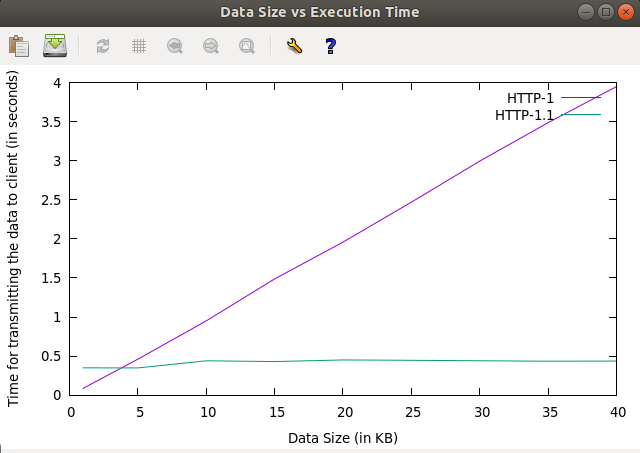
\includegraphics[width=6cm]{COP-1/Performance.png}
             \caption{Transmission Time of Data in HTTP-1.0 and HTTP-1.1}
             \label{fig:benchmaking}
      \end{figure}
  \end{enumerate}
  \section{Cites}
    \begin{enumerate}
        \item Socket programming : http://beej.us/guide/bgnet/
        \item https://tools.ietf.org/html/rfc1945
        \item https://tools.ietf.org/html/rfc2616
    \end{enumerate}
\end{document}
